
%%%
% Discussion of how each strategy was used as a separate starting point
%%%

\subsubsection*{Policy Initialization}
\label{sec:findings-expts-starts}

%%%
Since a desired outcome of the learning process was to be able to use the
generated strategy graphs to tell how a hand should be played in a
certain score position,
a comparison was made between the produced agent and pure strategies
on a database of choices made by humans.
%
The website Daily Cribbage Hand
prompts its users with
a set of dealt cards,
their score,
their opponent's score,
and an indication of whether or not the player is the dealer for the round
\cite{dailycribbagehand}.
%
With this prompt,
the user then decides which cards they would
keep in the given scenario.
%%%

%%%
With access to recorded answers from this website,
the agent's choices could be compared
to how humans ranked the choice.
%to those made by humans in the same situation.
%
For each of the approximately 3600 usable records,
the choice the agent made was compared against those made by the users of the
website.
%%%

%%%
The results of this comparison,
seen in Table~\ref{tab:expts-starts-human},
show that the agent trained in Round 2's losers' bracket chooses the same
set of cards as the human users only marginally more often than an agent with 
randomly allocated weights.
%
To approximately half of the prompts,
the trained agent chooses the same answer as most humans;
in almost 78 percent of the situations,
the answer given by the agent is within the top three most common human answers.
%
Additionally,
most pure strategies,
created by setting their weight to 1 while all other strategies are set to 0,
performed worse than the trained agent.
%
Notable exceptions to this trend are the \handmaxposs\ and \handmaxavg\ 
strategies,
suggesting that in more situations than the agent,
the typical human player will play according to what points can be expected
to be gained from the cut card.
%
Interestingly,
the \handmaxposs\ strategy's presence as the second most common pure strategy
used indicates a significant degree of risk-taking present in the users'
responses.
%
According to user comments,
this increased riskiness in play
may be a result of some users attempting to maximize points of the hand,
without the responsibility to actually play the resulting game,
and may not be entirely representative of actual in-game choices.
%%%

%%%
As a result of this finding,
some of these strategies were used as initial weights to the learning process
in order to determine if the agent could learn to fine-tune a policy starting
from a reasonable assertion of good game-play
as well as learn to discount demonstrably poor strategies.
%
Since the update mechanism for weights relies upon renormalization of a vector
which as been rewarded or punished,
no modifications would occur in the case of punishment of a completely pure strategy
since no other weights would have the chance to increase.
%
Therefore,
the pure strategies used before were slightly modified
such that each other
element of the \wvec\ vector would have a small initial value which could be
increased when this semi-pure strategy was punished.
%
Two agents,
each initialized with the same semi-pure strategy,
were played against each other for a million games,
with only a single agent updating its weights.
%%%


\begin{table}

	\begin{tabular}{|r|c|c|c|p{4cm}|}
		\hline
		\textbf{Strategy} & \textbf{Top 1} & \textbf{Top 2} & \textbf{Top 3}
			& \textbf{Percentage in Top 3 Human Choices} \\
		\hline
		\peggingminavggiven & 160 & 303 & 458 & 12.64 \\\hline
		\peggingmaxmedgained & 268 & 519 & 796 & 21.97 \\\hline
		\peggingmaxavggained & 347 & 650 & 963 & 26.58 \\\hline
		\cribminavg & 380 & 177 & 1081 & 29.84 \\\hline
		\handmaxmin & 1576 & 2288 & 2666 & 73.59 \\\hline
		\textbf{Random} & \textbf{1581} & \textbf{2318} & \textbf{2759} &
			\textbf{76.15} \\\hline
		\handmaxmed & 1649 & 2353 & 2768 & 76.40 \\\hline
		\textbf{Trained} & \textbf{1706} & \textbf{2426} & \textbf{2821} &
			\textbf{77.86} \\\hline
		\handmaxposs & 1677 & 2433 & 2847 & 78.58 \\\hline
		\handmaxavg & 2066 & 2828 & 3168 & 87.44 \\\hline
	\end{tabular}
	% total = 3623
	\caption{
		Number of times the agent using a given strategy chose the same cards as
		the most common choice by human users
		according to 3623 total parsable records obtained from
		\cite{dailycribbagehand}.
		The columns labeled ``Top X'' display the number of times the given
		strategy's choice was within the top X choices of the user base.
		%if at least that many different choices were made
		In this table,
		\textbf{Random} is from the best result of five agents which each used
		independently randomly allocated weights
		and
		\textbf{Trained} uses an agent trained from Round 2 for one million
		games.
	}
	\label{tab:expts-starts-human}
\end{table}



\paragraph*{Results}

%%%%
%There are very two interesting trends that arise from starting from nearly pure
%strategies.
%%
%The first is that the starting strategy is,
%at least for those tested,
%the dominant strategy in winning positions.
%%
%The second is what learning occurs in losing positions.
%%%%

%%%
The comparison of different strategies' development after training
(Figure~\ref{fig:findings-expts-sanitycheck-matrix})
shows the agent learning applicable policies
for both winning and losing positions.
%
In the winning positions of the strategy graphs,
the starting strategy is further strengthened to dominance.
%
The purely mathematical operation of overcoming such an initially heavily
weighted strategy requires many games to explore enough
and perform better than the starting strategy
to be rewarded;
%
the explored combination of cards, itself,
may coincide with the starting strategy
already occupying these positions,
further increasing the difficulty.
%
Additionally,
since the opponent is a static agent always using the same starting
semi-pure strategy and never training these weights,
playing a similar strategy ensures a similar resulting position.
%
When already in the lead,
this is desirable as the agent will likely continue to be in a winning position
and closer to the goal score of 121.
%
An intriguing counter to this pattern of dominance in winning positions
is the \handmaxavg\ strategy
which yields some control of winning positions to \handmaxmed.
%
After normal training procedures,
this space is occupied by \handmaxmin,
which, characteristically, would not allow a larger gap to develop.
%not allowing a larger gap to develop.
%%%

%%%
In losing positions,
the agent develops a reasonable counter policy
to the given semi-pure opponent.
%
For instance,
when faced with \handmaxmin\ which will always play safe,
the agent learns to swing for the fences by playing according to \handmaxposs\ 
when it is losing
since the opponent will not be taking any risks itself
and risk is the only way to make up ground.
%
Similarly,
the agent learns that the best way to recover from a losing position
against \handmaxavg,
which plays to expectations and avoids unnecessary risk,
is to mostly play safely according to \handmaxmin.
%
As a counter to the dominance of a single strategy in the losing positions,
starting with \handmaxposs\ leads to a losing strategy
shared between \handmaxavg\ and \handmaxmed.
%
This is because either of these two strategies is likely to recover ground
against an agent which always tries to get the maximum amount of points
with no regard for the likelihood of this outcome.
%%%

% fig:findings-expts-sanitycheck-matrix
\begin{figure}
\centering

\begin{tabular}{ l l l l l l } %    c}
	%                    label
	%  l            | l1   l2   l3   l4
	%  a   ---------+-------------------
	%  b   starting | a1 | a2 | a3 | a4
	%  e   strat    | b1 | b2 | b3 | b4
	%  l   ...
	& & \multicolumn{4}{c}{\textit{Strategy}} \\
	& & \handmaxmin & \handmaxavg & \handmaxposs & \handmaxmed \\
	%\cline{3-6}
	\multirow{7}{*}{
	\rotatebox{90}{
	\parbox[c]{6.5cm}{
		\textit{Starting Strategy}
	}
	}
	}
	%
	& \rotatebox[origin=c]{90}{\handmaxmin}
		&\parbox[c]{1em}{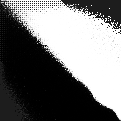
\includegraphics[width=2.5cm]{images/findings/experiments/starting_points/matrix_handmaxmin_handmaxmin.png}}
		&\parbox[c]{1em}{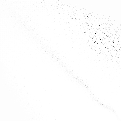
\includegraphics[width=2.5cm]{images/findings/experiments/starting_points/matrix_handmaxmin_handmaxavg.png}}
		&\parbox[c]{1em}{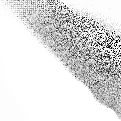
\includegraphics[width=2.5cm]{images/findings/experiments/starting_points/matrix_handmaxmin_handmaxposs.png}}
		&\parbox[c]{1em}{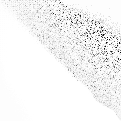
\includegraphics[width=2.5cm]{images/findings/experiments/starting_points/matrix_handmaxmin_handmaxmed.png}}
		%&
	\\ & & & & & \\
	%
	& \rotatebox[origin=c]{90}{\handmaxavg}
		&\parbox[c]{1em}{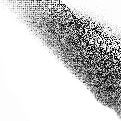
\includegraphics[width=2.5cm]{images/findings/experiments/starting_points/matrix_handmaxavg_handmaxmin.png}}
		&\parbox[c]{1em}{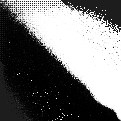
\includegraphics[width=2.5cm]{images/findings/experiments/starting_points/matrix_handmaxavg_handmaxavg.png}}
		&\parbox[c]{1em}{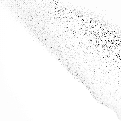
\includegraphics[width=2.5cm]{images/findings/experiments/starting_points/matrix_handmaxavg_handmaxposs.png}}
		&\parbox[c]{1em}{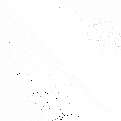
\includegraphics[width=2.5cm]{images/findings/experiments/starting_points/matrix_handmaxavg_handmaxmed.png}}
		%&\parbox[c]{1em}
	\\& & & & & \\
	%
	& \rotatebox[origin=c]{90}{\handmaxposs}
		&\parbox[c]{1em}{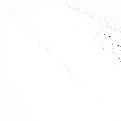
\includegraphics[width=2.5cm]{images/findings/experiments/starting_points/matrix_handmaxposs_handmaxmin.png}}
		&\parbox[c]{1em}{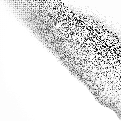
\includegraphics[width=2.5cm]{images/findings/experiments/starting_points/matrix_handmaxposs_handmaxavg.png}}
		&\parbox[c]{1em}{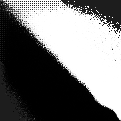
\includegraphics[width=2.5cm]{images/findings/experiments/starting_points/matrix_handmaxposs_handmaxposs.png}}
		&\parbox[c]{1em}{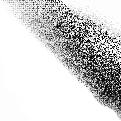
\includegraphics[width=2.5cm]{images/findings/experiments/starting_points/matrix_handmaxposs_handmaxmed.png}}
		%&\parbox[c]{1em}
	\\& & & & & \\
	%
	& \rotatebox[origin=c]{90}{\handmaxmed}
		&\parbox[c]{1em}{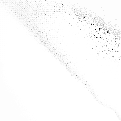
\includegraphics[width=2.5cm]{images/findings/experiments/starting_points/matrix_handmaxmed_handmaxmin.png}}
		&\parbox[c]{1em}{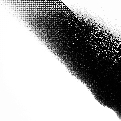
\includegraphics[width=2.5cm]{images/findings/experiments/starting_points/matrix_handmaxmed_handmaxavg.png}}
		&\parbox[c]{1em}{
\includegraphics[width=2.5cm]{images/findings/experiments/starting_points/matrix_handmaxmed_handmaxposs.png}}
		&\parbox[c]{1em}{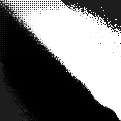
\includegraphics[width=2.5cm]{images/findings/experiments/starting_points/matrix_handmaxmed_handmaxmed.png}}
		%&\parbox[c]{1em}
	\\
\end{tabular}

\caption{}
\label{fig:findings-expts-sanitycheck-matrix}
\end{figure}


%%%
As this experiment showed promise in an agent potentially learning
to out-play its opponent,
an agent trained with a beginning pure strategy of \handmaxavg\ was played
against its previous iterations in several 10,000-game tournaments.
%
The results,
depicted in Figure~\ref{fig:expts-sanitycheck-spreads}
show a steady decrease in performance as training proceeds.
%
Earlier iterations,
closer to the semi-pure \handmaxavg\ strategy,
perform better than the trained agents.
%
Without further context,
it would appear that \handmaxavg\ is simply a good strategy which is difficult
enough to overcome,
so the training framework is forcing an adaptation
unnecessarily and undesirably.
%
However,
as the strategy graphs developed against a static semi-pure \handmaxavg\ 
opponent match those developed against a random agent
(Figure~\ref{fig:expts-sanitycheck-strats}),
this conclusion is unfounded.
%
If the \handmaxavg\ strategy were clearly superior to others,
then very little modification would be made by the agent.
%
Instead,
the losing states still drifted away from the starting strategy.
%
The only conclusions that can be made from this data are that
losing positions are fundamentally difficult to recover from
and that
cribbage involves much more than is encapsulated by the small set of
strategies with which the agent has been programmed.
%%%

% fig:expts-sanitycheck-spreads[-{a,b}]
% Point spreads for two runs of blah

\begin{figure}
\center

% TODO: actual images

\begin{subfigure}[t]{0.45\textwidth}
	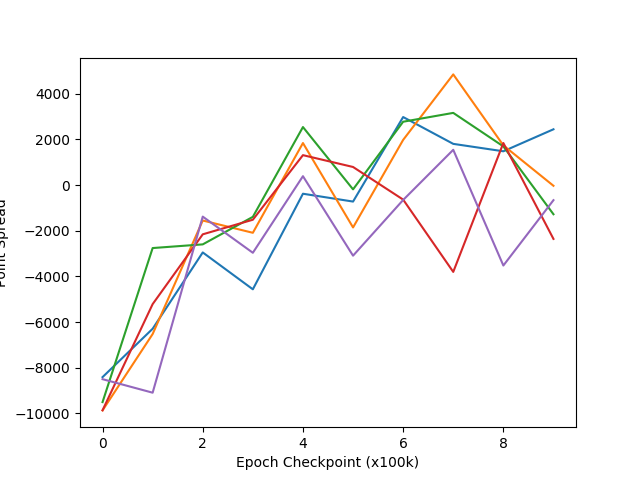
\includegraphics[width=\linewidth]{images/findings/experiments/starting_points/tourny_a.png}
	\caption{
		A trained agent starting from a semi-pure \handmaxavg\ strategy
		plays against previous iterations of itself.
	}
	\label{fig:expts-sanitycheck-spreads-a}
\end{subfigure}
~
\begin{subfigure}[t]{0.45\textwidth}
	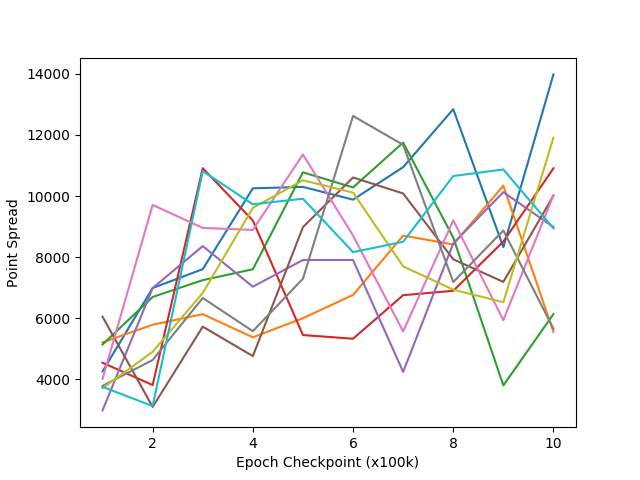
\includegraphics[width=\linewidth]{images/findings/experiments/starting_points/tourny_b.png}
	\caption{
		An agent using a semi-pure \handmaxavg\ strategy
		plays the epoch checkpoints of an agent which has been trained
		against this strategy.
	}
	\label{fig:expts-sanitycheck-spreads-b}
\end{subfigure}

\caption{
	Point spreads of several 10,000-game tournaments
	between agents of varying training levels
	when started with set of semi-pure \handmaxavg\ strategy weights.
}
\label{fig:expts-sanitycheck-spreads}
\end{figure}


%%%%%%
%%%Furthermore,
%%%as the agents were previously each trained against different pure strategies,
%%%the ability to improve a basic policy to overcome a randomly-weighted agent,
%%%rather than to learn a policy from scratch,
%%%was tested by training an agent starting with a semi-pure
%%%\handmaxavg\ strategy against an unlearning agent with random weights.
%%%%
%%%The results of this further training,
%%%seen in Figure~\ref{fig:expts-sanitycheck-strats},
%%%show that the same behavioral trends are learned by an
%%%agent starting with a semi-pure \handmaxavg\ strategy 
%%%when the opponent is random
%%%as well as when the opponent follows the same semi-pure strategy.
%%%%%%

% fig:expts-sanitycheck-strats

\begin{figure}
\center

% TODO: actual images

	\begin{subfigure}[t]{0.22\textwidth}
		%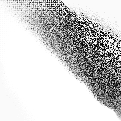
\includegraphics[width=\textwidth]{images/findings/experiments/starting_points/hand_max_min.png}
		\caption{\handmaxmin}
	\end{subfigure}
	~
	\begin{subfigure}[t]{0.22\textwidth}
		%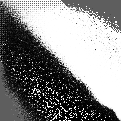
\includegraphics[width=\textwidth]{images/findings/experiments/starting_points/hand_max_avg.png}
		\caption{\handmaxavg}
	\end{subfigure}
	~
	\begin{subfigure}[t]{0.22\textwidth}
		%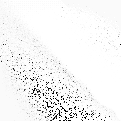
\includegraphics[width=\textwidth]{images/findings/experiments/starting_points/hand_max_med.png}
		\caption{\handmaxmed}
	\end{subfigure}
	~
	\begin{subfigure}[t]{0.22\textwidth}
		%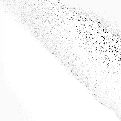
\includegraphics[width=\textwidth]{images/findings/experiments/starting_points/hand_max_poss.png}
		\caption{\handmaxposs}
	\end{subfigure}

	\begin{subfigure}[t]{0.22\textwidth}
		%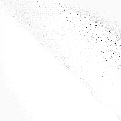
\includegraphics[width=\textwidth]{images/findings/experiments/starting_points/crib_min_avg.png}
		\caption{\cribminavg}
	\end{subfigure}
	~
	\begin{subfigure}[t]{0.22\textwidth}
		%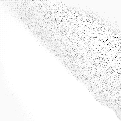
\includegraphics[width=\textwidth]{images/findings/experiments/starting_points/pegging_max_avg_gained.png}
		\caption{\peggingmaxavggained}
	\end{subfigure}
	~
	\begin{subfigure}[t]{0.22\textwidth}
		%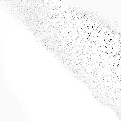
\includegraphics[width=\textwidth]{images/findings/experiments/starting_points/pegging_max_med_gained.png}
		\caption{\peggingmaxmedgained}
	\end{subfigure}
	~
	\begin{subfigure}[t]{0.22\textwidth}
		%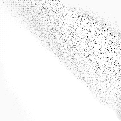
\includegraphics[width=\textwidth]{images/findings/experiments/starting_points/pegging_min_avg_given.png}
		\caption{\peggingminavggiven}
	\end{subfigure}

\caption{
	All final strategy strengths for an agent
	which started with a 70\% semi-pure \handmaxavg\ strategy
	and was trained against an agent with unchanging random weights
	for one million games
	when playing as the dealer.
}
\label{fig:expts-sanitycheck-strats}
\end{figure}


